%% Преамбула TeX-файла

% 1. Стиль и язык
\documentclass[utf8x, 12pt]{G7-32} % Стиль (по умолчанию будет 14pt)

% Остальные стандартные настройки убраны в preamble.inc.tex.
\sloppy

% Настройки стиля ГОСТ 7-32
% Для начала определяем, хотим мы или нет, чтобы рисунки и таблицы нумеровались в пределах раздела, или нам нужна сквозная нумерация.
\EqInChapter % формулы будут нумероваться в пределах раздела
\TableInChapter % таблицы будут нумероваться в пределах раздела
\PicInChapter % рисунки будут нумероваться в пределах раздела

% Добавляем гипертекстовое оглавление в PDF
\usepackage[
bookmarks=true, colorlinks=true, unicode=true,
urlcolor=black,linkcolor=black, anchorcolor=black,
citecolor=black, menucolor=black, filecolor=black,
]{hyperref}

\AfterHyperrefFix

\usepackage{microtype}% полезный пакет для микротипографии, увы под xelatex мало чего умеет, но под pdflatex хорошо улучшает читаемость

% Тире могут быть невидимы в Adobe Reader
\ifInvisibleDashes
\MakeDashesBold
\fi

\usepackage{graphicx}   % Пакет для включения рисунков

% С такими оно полями оно работает по-умолчанию:
% \RequirePackage[left=20mm,right=10mm,top=20mm,bottom=20mm,headsep=0pt,includefoot]{geometry}
% Если вас тошнит от поля в 10мм --- увеличивайте до 20-ти, ну и про переплёт не забывайте:
\geometry{right=20mm}
\geometry{left=30mm}
\geometry{bottom=20mm}
\geometry{ignorefoot}% считать от нижней границы текста


% Пакет Tikz
\usepackage{tikz}
\usetikzlibrary{arrows,positioning,shadows}

% Произвольная нумерация списков.
\usepackage{enumerate}

% ячейки в несколько строчек
\usepackage{multirow}

% itemize внутри tabular
\usepackage{paralist,array}

%\setlength{\parskip}{1ex plus0.5ex minus0.5ex} % разрыв между абзацами
\setlength{\parskip}{1ex} % разрыв между абзацами
\usepackage{blindtext}

% Центрирование подписей к плавающим окружениям
%\usepackage[justification=centering]{caption}


% Настройки листингов.
\ifPDFTeX
% 8 Листинги

\usepackage{listings}

% Значения по умолчанию
\lstset{
  basicstyle= \footnotesize,
  breakatwhitespace=true,% разрыв строк только на whitespacce
  breaklines=true,       % переносить длинные строки
%   captionpos=b,          % подписи снизу -- вроде не надо
  inputencoding=koi8-r,
  numbers=left,          % нумерация слева
  numberstyle=\footnotesize,
  showspaces=false,      % показывать пробелы подчеркиваниями -- идиотизм 70-х годов
  showstringspaces=false,
  showtabs=false,        % и табы тоже
  stepnumber=1,
  tabsize=4,              % кому нужны табы по 8 символов?
  frame=single
}

% Стиль для псевдокода: строчки обычно короткие, поэтому размер шрифта побольше
\lstdefinestyle{pseudocode}{
  basicstyle=\small,
  keywordstyle=\color{black}\bfseries\underbar,
  language=Pseudocode,
  numberstyle=\footnotesize,
  commentstyle=\footnotesize\it
}

% Стиль для обычного кода: маленький шрифт
\lstdefinestyle{realcode}{
  basicstyle=\scriptsize,
  numberstyle=\footnotesize
}

% Стиль для коротких кусков обычного кода: средний шрифт
\lstdefinestyle{simplecode}{
  basicstyle=\footnotesize,
  numberstyle=\footnotesize
}

% Стиль для BNF
\lstdefinestyle{grammar}{
  basicstyle=\footnotesize,
  numberstyle=\footnotesize,
  stringstyle=\bfseries\ttfamily,
  language=BNF
}

% Определим свой язык для написания псевдокодов на основе Python
\lstdefinelanguage[]{Pseudocode}[]{Python}{
  morekeywords={each,empty,wait,do},% ключевые слова добавлять сюда
  morecomment=[s]{\{}{\}},% комменты {а-ля Pascal} смотрятся нагляднее
  literate=% а сюда добавлять операторы, которые хотите отображать как мат. символы
    {->}{\ensuremath{$\rightarrow$}~}2%
    {<-}{\ensuremath{$\leftarrow$}~}2%
    {:=}{\ensuremath{$\leftarrow$}~}2%
    {<--}{\ensuremath{$\Longleftarrow$}~}2%
}[keywords,comments]

% Свой язык для задания грамматик в BNF
\lstdefinelanguage[]{BNF}[]{}{
  morekeywords={},
  morecomment=[s]{@}{@},
  morestring=[b]",%
  literate=%
    {->}{\ensuremath{$\rightarrow$}~}2%
    {*}{\ensuremath{$^*$}~}2%
    {+}{\ensuremath{$^+$}~}2%
    {|}{\ensuremath{$|$}~}2%
}[keywords,comments,strings]

% Подписи к листингам на русском языке.
\renewcommand\lstlistingname{Листинг}
\renewcommand\lstlistlistingname{Листинги}

\else
\usepackage{local-minted}
\fi

% Полезные макросы листингов.
% Любимые команды
\newcommand{\Code}[1]{\textbf{#1}}


% Стиль титульного листа и заголовки
%
%\NirEkz{Экз. 3}                                  % Раскоментировать если не требуется
%\NirGrif{Секретно}                % Наименование грифа

%\gosttitle{GostRV15-110}       % Шаблон титульной страницы, по умолчанию будет ГОСТ 7.32-2001, 
% Варианты GostRV15-110 или Gost7-32 
 
\NirOrgLongName{Министерство общего и профессионального образования \\
Российской Федерации\par
ПЕТРОЗАВОДСКИЙ ГОСУДАРСТВЕННЫЙ УНИВЕРСИТЕТ \\
Физико-технический институт \\
Кафедра информационно-измерительных систем и физической электроники
}                                           %% Полное название организации

\NirUdk{УДК № 004.733}
\NirGosNo{№ госрегистрации 00000000000}
%\NirInventarNo{Инв. № ??????}

%\NirConfirm{Согласовано}                  % Смена УТВЕРЖДАЮ
\NirBoss[.49]{Проректор университета\\по научной работе}{И.И. Иванов}            %% Заказчик, утверждающий НИР


%\NirReportName{Научно-технический отчет}   % Можно поменять тип отчета
%\NirAbout{О составной части \par опытно-конструкторской работы} %Можно изменить о чем отчет

%\NirPartNum{Часть}{1}                      % Часть номер

%\NirBareSubject{}                  % Убирает по теме если раскоментить

% \NirIsAnnotacion{АННОТАЦИОННЫЙ }         %% Раскомментируйте, если это аннотационный отчёт
%\NirStage{промежуточный}{Этап \No 1}{} %%% Этап НИР: {номер этапа}{вид отчёта - промежуточный или заключительный}{название этапа}
%\NirStage{}{}{} %%% Этап НИР: {номер этапа}{вид отчёта - промежуточный или 

\Nir{Применение беспроводных технологии LPWAN с низким энергопотреблением в концепции интернета вещей}

\NirSubject{Применение технологии LoRa в концепции IoT}                          % Наименование темы
%\NirFinal{}                        % Заключительный, если закоментировать то промежуточный
%\finalname{итоговый}               % Название финального отчета (Заключительный) 
%\NirCode{Шифр\,---\,САПР-РЛС-ФИЗТЕХ-1} % Можно задать шифр как в ГОСТ 15.110
\NirCode{}

\NirManager{Доцент, кандидат физ.-мат. наук, доцент}{А. П. Мощевикин} %% Название руководителя
%\NirIsp{Руководитель темы}{Г.А. Кабакович} %% Название руководителя

%\NirYear{1999}%% если нужно поменять год отчёта; если закомментировано, ставится текущий год
\NirTown{Петрозаводск}                           %% город, в котором написан отчёт



\begin{document}

\frontmatter % выключает нумерацию ВСЕГО; здесь начинаются ненумерованные главы: реферат, введение, глоссарий, сокращения и прочее.

%\maketitle %создает титульную страницу


%\begin{executors}
%\personalSignature{Первый исполнитель}{ФИО}
%
%\personalSignature{Второй исполнитель}{ФИО}
%\end{executors}


%\listoffigures                         % Список рисунков

%\listoftables                          % Список таблиц

%\NormRefs % Нормативные ссылки 
% Команды \breakingbeforechapters и \nonbreakingbeforechapters
% управляют разрывом страницы перед главами.
% По-умолчанию страница разрывается.

% \nobreakingbeforechapters
% \breakingbeforechapters

% Также можно использовать \Referat, как в оригинале
\begin{abstract}

    Отчет содержит \pageref{LastPage}\,стр.%
    \ifnum \totfig >0
    , \totfig~рис.%
    \fi
    \ifnum \tottab >0
    , \tottab~табл.%
    \fi
    %
    \ifnum \totbib =1
    , \totbib~источник%
    \else
    \ifnum \totbib >1
    \ifnum \totbib <5
    , \totbib~источника%
    \else
    , \totbib~источников%
    \fi
    \fi
    \fi
    %
    \ifnum \totapp >0
    , \totapp~прил.%
    \fi
    
	Ключевые слова: LoRa, Интернет вещей, M2M, беспроводные технологии 
передачи данных, открытое программное обеспечение, разработка ПО.

	Данная работа ставит перед собой цель изучения технологии беспроводной передачи данных LoRa в контексте её использования в Интернете вещей.

	В работе кратко отображено современное состояние Интернета вещей 
и беспроводных технологий передачи небольших по объёму данных на дальние 
расстояние и с низким энергопотреблением.
	Рассмотрен способ использования принципа открытого программного обеспечения для создания конечных устройств в сети LoRaWAN.


    \nocite{*}

\end{abstract}

%%% Local Variables: 
%%% mode: latex
%%% TeX-master: "rpz"
%%% End: 


\tableofcontents

\printnomenclature % Автоматический список сокращений

\Introduction

С ростом информационных технологий и коммуникаций в XXI веке новые тенденции проявляются в виде интеллектуальной обработки больших массивов данных (Big Data) и Интернете вещей (IoT или IdC). 
Интернет не только позволил объединить людей, но также и устройства, датчики в сложные системы. 
Так появляется термин «Интернет вещей», который соответствует соединению различных устройств с Интернетом, генерирующие данные в реальном времени. 
Так называемые сети с низким энергопотреблением и большим покрытием (LPWA) являются мостом к Интернету Вещей, разработанные с целью заполнить брешь в технологиях с низким энергопотреблением, большим покрытием и низкой стоимостью. 
Одной из лидирующих технологии LPWAN является LoRaWAN. Она и станет объектом рассмотрения данной работы.

Целями данной работы являются:


\begin{itemize}
	\item изучить возможные применения технологии в контексте развития Интернета вещей;
	\item сравнить открытый стандарт LoRaWAN с другими технологиями беспроводной передачи данных, таких как SigFox, LTE, Стриж и т.д;
	\item оценить характеристики энергопотребления и зону покрытия в городской среде для радиоприёмника LoRa SX1278 в разных режимах работы;
	\item создать и задокументировать программное обеспечение для работы с SX1278 в связке с STM32L476, используя инструменты открытого программного обеспечения.
\end{itemize}

\Abbrev{LPWAN}{Low-power Wide-aread Network ""--- энергоэффективная сеть дальнего радиуса действия}
\Abbrev{CSS}{Chirp spread spectrum ""--- линейная частотная модуляция}
\Abbrev{ISM}{industrial, scientific and medical radio bands""--- международные зарезервированные частотные дипазоны}
\Abbrev{NGN}{Next Generation Network ""--- сеть последующих поколений}
\Abbrev{IoT}{с англ. \textit{Internet of Things} в переводе ""--- \textit{``Интернет вещей''}} 
\Abbrev{LTE}{Long Term Evolution ""--- долгосрочное развитие}
%\Abbrev{API}{Application Programming Interface ""--- внешний интерфейс взаимодействия с приложением}

\Define{Интернет}{глобальная вычислительная сеть. Является самой большой компьютерной сетью в мире. Построена на базе стека протоколов TCP/IP}
\Define{Сетевой протокол}{соглашение о наборе правил, повзоляющих проводить соединение и обмен данными между двумя и более устройствами, подключенным к сети}
\Define{Сеть последующих поколений (СПП) (Next generation network)}{Сеть с пакетной коммутацией, пригодная для предоставления услуг электросвязи и для использования нескольких широкополосных технологий транспортировки с ключенной функцией QoS, в который связанные с обслуживанием функции не зависят от примененных технологий, обепечивающих транспортировку}



\mainmatter % это включает нумерацию глав и секций в документе ниже

\chapter{Аналитический обзор}
\label{cha:analysis}
%
% % В начале раздела  можно напомнить его цель
%
%В данном разделе анализируется и классифицируется существующая всячина и пути создания новой всячины. А вот отступ справа в 1 см. "--- это хоть и по ГОСТ, но ведь диагноз же...

%%%%%%%%%%%%%%%%%%%%%%%%%%%%%%%%%%%%%%%%%%%%%%%%%%%%%%%%%%%%%%%%%%%%%%%%%%%%%%%%%%%%%%%%%%%%%%%%%%%%%%%%%%%%%%%%

\section{Что такое Интернет вещей}

Интернет вещей (англ. \textit{IoT}, \textit{Internet of Things}) ""--- это методология вычислительной сети физических объектов (``\textit{вещей}''), имеющих встроенную поддержку технологий передачи данных для их взаимодействия, а также для взаимодействия с внешней средой.
Эта методология рассматривает Интернет вещей как явление, способное перестроить культурные и экономические процессы, всё больше исключая человека из них.
Влияние существующего Интернета на сферы образования, коммуникации, бизнеса, науки и политики позволяет говорить о том, что Интернет является одним из важнейших и мощнейших изобретений в истории человечества\cite{evans2011internet}.
Интернет вещей стоит рассматривать как новую ветвь эволюции Интернета, где каждый предмет в поле зрения человека может быть оснащён датчиками, сенсорами, устройством управления и модулем передачи данных для общения со всем миром.

Как известно, большинство великих изобретений человечества потребовали десятки и даже сотни лет на переход от простых по форме представлений до сложных систем.
От создания предпосылок, до массового внедрения Интернета ушло почти четверть века, однако похоже что для Интернета вещей на то же самое потребуется существенно меньше времени \cite{chernyak2013}.
Международный союз связи (МСЭ) и Европейский Союз определили Интернету вещей главенствующую роль в дальнейшем развитии отрасли инфокоммуникации. 
По расчетам консалтингового подразделения Cisco IBSG (см. рис. \ref{fig:iotandpeople}) в промежутке между 2008 и 2009 годами, количество устройств, подключенных к интернету, превысило количество людей, и к 2020 году количество подключенных устройств достигнет 50 миллиардов\cite{evans2011internet} (по другим данным\cite{denise2014} ""--- 25 миллиардов).
Таким образом, в настоящее время происходит переход от ``Интернета людей'' к ``Интернету вещей''.
Хотя данная концепция на международном уровне уже обретает черты сформировавшейся технологии, для неё ведутся активные работы в области стандартизации компонентов, архитектуры и приложений.
Количество мнений о том как будет построен Интернет вещей очень велико. 
Это подтверждается большим разнообразием предлагаемых технологий для создания LPWAN сетей на рынке.

\begin{figure}
  \centering
  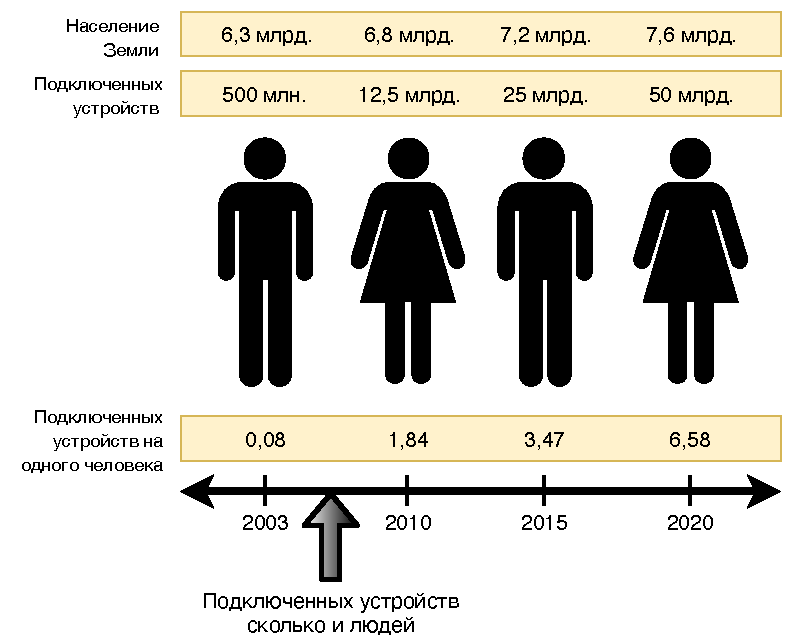
\includegraphics[width=0.8\textwidth]{inc/img/IoTAndPeople}
	\caption{Временная шкала изменения количества людей и предметов, подключенных к интернет \cite{evans2011internet}}
  \label{fig:iotandpeople}
\end{figure}

%Кстати, про картинки. Во-первых, для фигур следует использовать \texttt{[ht]}. Если и после этого картинки вставляются <<не по ГОСТ>>, т.е. слишком далеко от места ссылки, "--- значит у вас в РПЗ \textbf{слишком мало текста}! Хотя и ужасный параметр \texttt{!ht} у окружения \texttt{figure} тоже никто не отменял, только при его использовании документ получается страшный, как в ворде, поэтому просьба так не делать по возможности.

\subsection{Базовые принципы Интернета вещей}

Интернет вещей основывается на трёх базовых принципах\cite{roslyakov2014}.
\begin{enumerate}
	\item повсеместно распространенная инфраструктура;
	\item глобальная идентификация каждого объекта;
	\item возможность каждого физического объекта отправлять и получать данные, посредством локальной сети или сети Интернет, к которой он подключен.
\end{enumerate}

Наиболее важными отличиями Интернета вещей от интернета людей являются:
\begin{itemize}
	\item фокус на считывание информации, а не на коммуникациях;
	\item на порядки большее число подключенных к сети объектов;
	\item потребность в создании новых стандартов;
	\item намного меньше размеры объектов и скорости передачи данных;
	\item фокус не на человеке, а на вещах;
\end{itemize}

Концепция сетей следующего поколения NGN предполагала возможность коммуникаций людей в любой точке пространства и времени.
Концепция интернета вещей включает ещё одно направление ""--- коммуникация любых вещей или устройств (рис. \ref{fig:iotconcept})

\begin{figure}
  \centering
  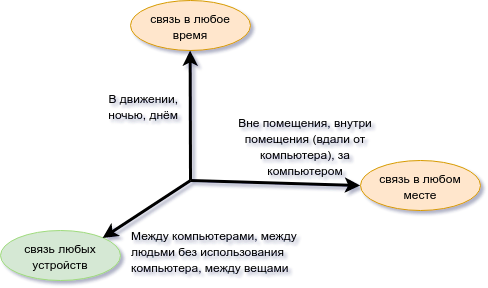
\includegraphics[width=0.8\textwidth]{inc/img/IoTConcept}
	\caption{Новое направление коммуникаций, реализуемой Интернетом вещей\cite{itutiot2012}}
  \label{fig:iotconcept}
\end{figure}

Согласно принятым в МСЭ-Т представлениям о отображении физических и виртуальных вещей, виртуальные вещи могут обходится без их физического соответствия, в то время как каждой физической вещи соответствует минимум один объект в виртуальном пространстве (см. рис. \ref{fig:physvirtworld}).  

Рекомендация Y.2060 от МСЭ-Т описывает различное сочетание способов соединений.
МСЭ-Т рассматривает множество сетевых технологий, как потенциально пригодных для приложений Интернета вещей, а именно: глобальные сети, локальные сети, ячеистые (mesh) сети и беспроводные самоорганизующиеся (ad-hoc) сети.

\begin{figure}
  \centering
  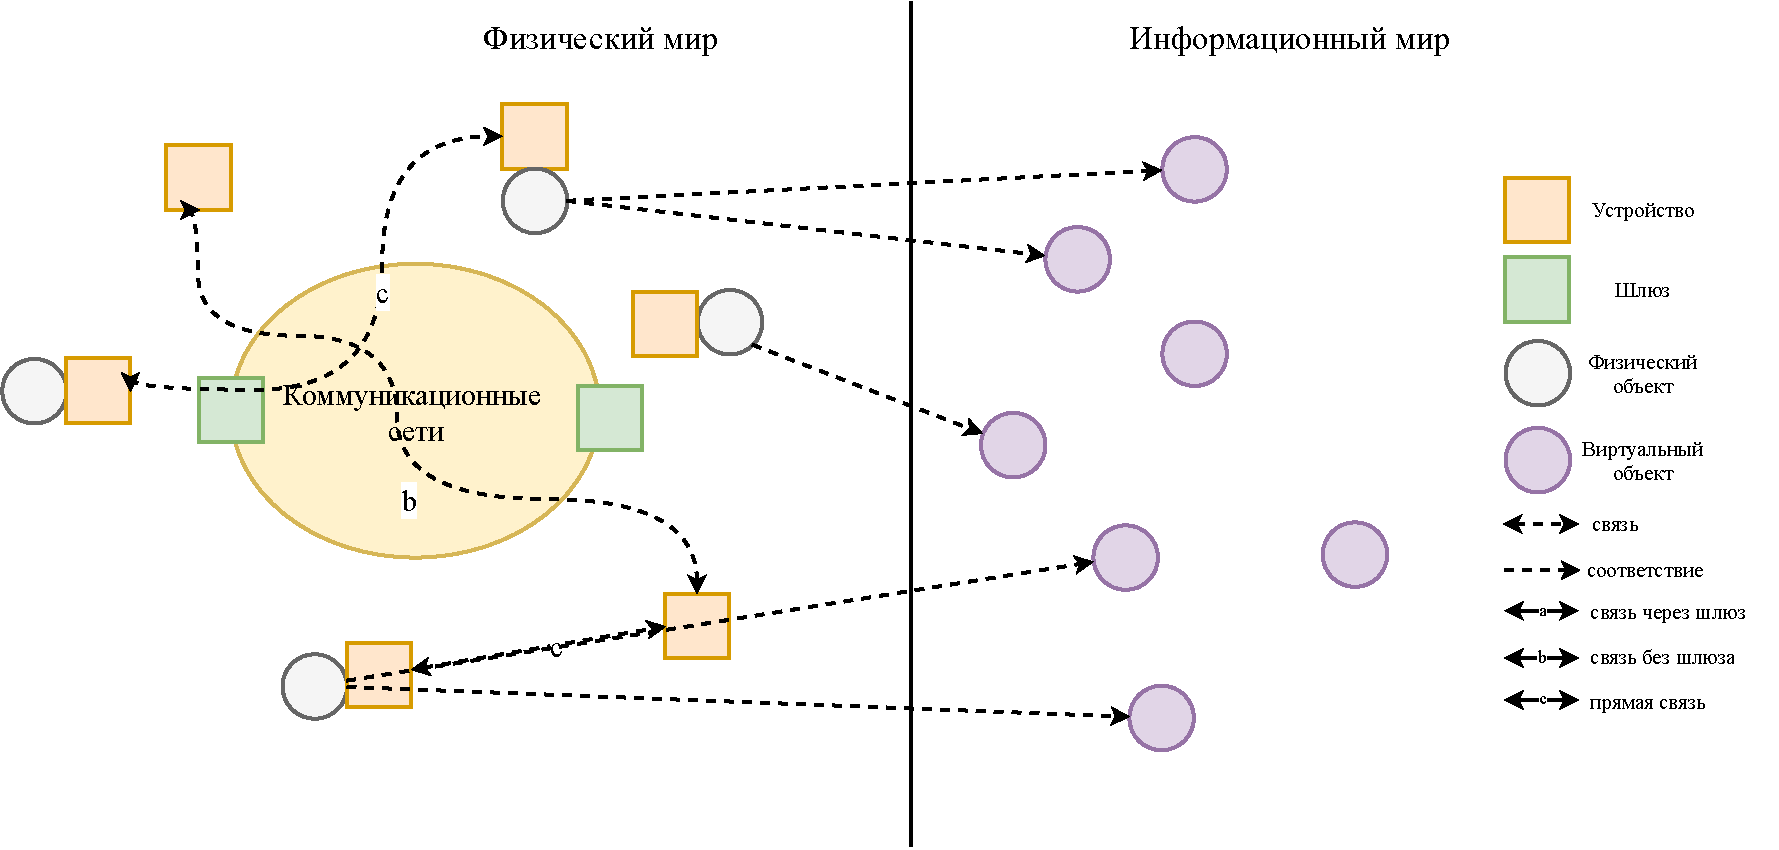
\includegraphics[width=0.9\textwidth]{inc/img/realvirtualthings}
	\caption{Отображение физических и виртуальных вещей\cite{itutiot2012}}
  \label{fig:physvirtworld}
\end{figure}

\subsection{Основные характеристики Интернета вещей}

IoT, имеет следующие характеристики:

\begin{itemize}
	\item возможность установления соединений. Любую вещь можно соединить к Интернету вещей;
	\item гетерогенность: устройства в концепции Интернета вещей являются гетерогенными и базируются на различных аппаратных платформах и сетях. 
		Могут обмениваться информацией с другими устройствами, независимо от структуры сети и применяемых технологий транспортного уровня. 
		Примечательно, что современное состояние сети Интернет может удовлетворить этому лишь отчасти: пул адресов IPv4 исчерпан и большая часть устройств скрывается в локальных сетях за устройствами NAT, что противоречит изначальной концепции однородного интернета. 
		Решением может стать повсеместное использование протокола IPv6 в качестве протокола сетевого уровня. 
		Хотя внедрение этого протокола и затянулось, но уже к декабрю 2018 года ожидается, что 25\% всех Интернет доменов будет доступно через этот протокол\cite{pickard2017}.;
	\item огромное количество, одновременно подключенных, устройств к сети, которыми необходимо управлять, обмениваться данными. Произойдёт существенное увеличение долей обмена данными, инициированными устройствами, по сравнению с долей информационного обмена, инициированного людьми;
	\item динамические изменения структуры сети. Устройства будут свободно подключаться к сетям, менять своё местоположение, отключаться от сети и подключаться к новым устройствам. Подразумевается, что количество устройств в одной сети - переменная величина с течением времени;
\end{itemize}

Важной частью рекомендации от МСЭ-Т являются требования	предъявляемые к устройствам IoT. Любые технологии LPWAN, в том числе и LoRa, должны соответствовать этим требованиям для предоставления возможности их включения в инфраструктуру Интернета вещей:

\begin{itemize}
	\item предоставление автономных услуг: требуется что бы услуги могли предоставляться с помощью автоматической передачи, обработки и сбора данных вещей, основанных на правилах, задаваемых операторами или абонентами. Услуги могут зависеть от методов автоматизированной обработки и интеллектуального анализа данных;
	\item соединение на основе идентификатора: соединение с любой вещью в концепции Интернета вещей будет происходить на основе уникального идентификатора, которым обладает тот или иной объект. Отсюда выходит требование о создании универсального идентификатора (например адрес IPv6) для применения в гетерогенных сетях.
	\item функциональная совместимость: требуется обеспечение функциональной совместимости гетерогенных и распределенных систем в целях предоставления и потребления самый разных видов услуг;
	\item  возможности определения местоположения: требуется что бы в Интернете вещей обеспечивались услуги, на основе информации о местоположении объекта. Требуется что бы информация о местоположении вещей отслеживалась автоматически. Связь и услуги на основе местоположения могут быть ограничены законами и нормативными актами и должны соответствовать требованиям безопасности;
	\item безопасность в Интернете вещей: каждая вещь имеет соединение с сетью, что приводит к серьёзной угрозе безопасности, таким как угроза аутентичности, целостности и конфиденциальности как данных, так и услуг. Одним и важнейших требования к безопасности является необходимость объединения различных методов и принципов обеспечения безопасности множества устройств и сетей пользователей;
	\item защита неприкосновенности частной жизни: требуется, чтобы в IoT обеспечивалась неприкосновенность частной жизни. У многих вещей есть владельцы и эти вещи могут хранить личную информацию их владельцев. Необходимо обеспечить неприкосновенность частной жизни человека при сборе, обработке, анализе и передачи больших массивов информации вещами. Защита неприкосновенности частной жизни не должна служить препятствием для аутентификации источника данных;
	\item автоматическое конфигурирование: необходимо обеспечить возможность автоматического конфигурирования устройств, для возможности оперативной модификации программного обеспечения вещей, с целю повысить качество обслуживания клиентов, а также степень интеграции устройства с окружающим миром и сетью, не нарушая при этом, требования о безопасности и конфиденциальности.
	\item управляемость: возможность вмешательства человека в работу вещей при необходимости.
\end{itemize}

\subsection{Эталонная модель Интернета вещей}

Также была разработана эталонная модель интернета вещей, она показана на рисунке \ref{fig:iotetalon}.
Она включает в себя четыре уровня, а также возможности обеспечения безопасности и управления, которые связаны с этими четырьмя уровнями:

\begin{itemize}
	\item уровень приложения;
	\item уровень поддержки услуг и поддержки приложения;
	\item уровень сети;
	\item уровень устройства.
\end{itemize}

\begin{figure}
  \centering
  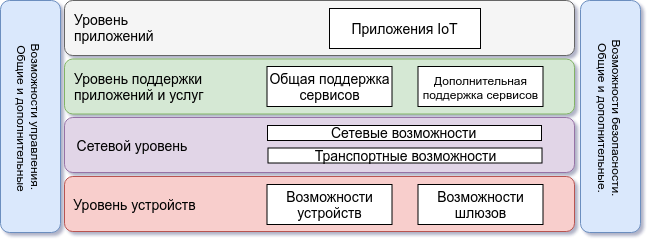
\includegraphics[width=\textwidth]{inc/img/iotetalon}
	\caption{Эталонная модель IoT\cite{itutiot2012}}
  \label{fig:iotetalon}
\end{figure}

\subsubsection{Уровень приложения}

Содержит само приложение IoT.

\subsubsection{Уровень поддержки услуг и поддержки приложений}

Данный уровень состоит из следующих двух групп возможностей:

\begin{itemize}
	\item общие возможности поддержки, или типовые возможности, которые могут использоваться приложениями Интернета вещей, такими как хранение или обработка данных.
	\item специализированные возможности поддержки или набор конкретных возможностей, предназначенных для удовлетворения требований разнообразных приложений.
\end{itemize}

\subsubsection{Уровень сети}

Существует два типа возможностей:

\begin{itemize}
	\item возможности организации сетей: предоставляет функции управления сетевыми соединениями;
	\item возможности транспортировки: предназначены для предоставления соединений для транспортировки информации в виде данных, относящихся к услугам и приложениям IoT, а также транспортировки информации управления и контроля, относящейся к IoT.
\end{itemize}

\subsubsection{Уровень устройства}

Этот уровень можно логически разделить на два вида возможностей:
\begin{itemize}
	\item возможности устройства. Это могут быть такие возможности, как: спящий режим и пробуждение, организация специальных сетей, прямое и непрямое взаимодействие устройства с сетью;
	\item возможности шлюза. Это возможность поддержки различных интерфейсов. Шлюза объединяют в себе различные сетевые интерфейсы, как проводные, так и беспроводные.
\end{itemize}

\subsubsection{Возможности управления}

Возможности управления IoT охватывают традиционные классы конфигурации, учета, безопасности и т.д.

Важнейшие возможности управления включают:
\begin{itemize}
	\item управление устройствами, диагностика, обновление, прошивка, управление рабочим состоянием устройства;
	\item управление топологией локальной сети;
	\item управление трафиком и перегрузками.
\end{itemize}

\subsubsection{Возможности обеспечения безопасности}

Есть два вида возможностей обеспечения безопасности: общие и специализированные.
Общие возможности не зависят от приложений и включают:
\begin{itemize}
	\item на уровне приложений: авторизацию, конфиденциальность, аутентификацию, целостность данных приложения, защиту неприкосновенности частной жизни, аудит безопасности;
	\item на уровне сети: авторизацию, аутентификацию, защиту конфиденциальности и целостности;
	\item на уровне устройства: аутентификацию, авторизацию, проверку целостности устройства, управление доступом, защиту целостности и конфиденциальности.
\end{itemize}

Специализированные возможности зависят от вида приложений и могут налагать дополнительные специфичные требования по безопасности.

%%%%%%%%%%%%%%%%%%%%%%%%%%%%%%%%%%%%%%%%%%%%%%%%%%%%%%%%%%%%%%%%%%%%%%%%%%%%%%%%%%%%%%%%%%%%%%%%%%%%%%%%%%%%%%%%
\newpage
\section{Обзор технологии LoRa} 

В данном разделе будет дан обзор на технологию LoRa от компании Semtech.
Будет кратко рассмотрены физический и уровень управления доступом к сети (MAC) LoRaWAN сетей.

\subsection{Стек протоколов LoRa}

\subsubsection{Физический уровень}

LoRa представляет собой технологию энергоэффективной сети дальнего радиуса действия, разрабатываемый организацией LoRa Alliance.
Данная технология нацелена на использование в устройствах с автономными источниками питания, где показатель энергопотребления является наиболее важным.
Технология LoRa описывает два независимых уровня протоколов: физический, с использование линейной частотной модуляцией (CSS); и протокол контроля доступа к среде (LoRaWAN), хотя системы коммуникации LoRa также реализуют специфичные сетевые архитектуры\cite{augustin2016}.

Физический уровень LoRa разработан компанией Semtech и он обеспечивает связь с низким энергопотреблением, низкой скоростью и большим радиусом действия.

\paragraph{Доступные частотные диапазоны} \hspace{0pt}\\

Физический уровень LoRa работает в различных субгигагерцовых частотных ISM диапазонах.
В различных странах приняты различные диапазоны частот, поэтому устройствам с LoRa необходимо самостоятельно выбирать используемый радиодиапазон для физического уровня, в зависимости от принятых местных соглашениях. 
Таблица \ref{tab:ismbands} описывает, принятые в различных странах, частотные диапазоны для строительства сетей связи.

\begin{table}[ht]
  \caption{Частотные диапазоны, принятые в разных странах}
  \begin{tabular}{|l|c|}
  \hline
	  Частотный диапазон & Страна\\
  \hline
	  EU 863-870 МГц ISM & Европейский союз\\
  \hline
	  EU 433 МГц ISM & Европейский союз\\
  \hline
	  RU 864-870 МГц ISM & Российская Федерация\\
  \hline
	  US 902-928 МГц ISM & США\\
  \hline
	  CH 779-787 МГц ISM & КНР\\
  \hline
  \end{tabular}
  \label{tab:ismbands}
\end{table}

В 2017 году был утвержден частотный план LoRa Alliance, в котором определены единые региональные параметры LoRaWAN, используемые на территории РФ.
Согласно этому плану, для РФ выделяется частотный диапазон шириной в 6 МГц, с максимальной шириной полосы частот в 125 кГц.
При этом для конечных устройств \textbf{обязательна} поддержка двух каналов с несущими 868,9 и 869,1 МГц/ DR0 до DR5 (см. таблицу \ref{tab:rudefchannels}).

% TODO: Про доступные частотные диапазоны можно написать больше

\begin{table}[ht]
  \caption{Стандартные каналы частотного диапазона RU864-870}
\begin{tabular}{|l|l|l|l|l|l|}
\hline
	Модуляция & \begin{tabular}[c]{@{}l@{}}Ширина \\ полосы\\ частот \\ {[}кГц{]}\end{tabular} & \begin{tabular}[c]{@{}l@{}}Несущая\\ {[}МГц{]}\end{tabular}& \begin{tabular}[c]{@{}l@{}}Пропускная\\ способность\\ FSK или \\ LoRa DR\end{tabular}& \begin{tabular}[c]{@{}l@{}}Кол-во\\ каналов\end{tabular} & \begin{tabular}[c]{@{}l@{}}Рабочий\\ цикл\end{tabular} \\ \hline
	\multicolumn{1}{|c|}{LoRa} & \multicolumn{1}{c|}{125}& \multicolumn{1}{c|}{\begin{tabular}[c]{@{}c@{}}868,9\\ 869,1\end{tabular}} & \multicolumn{1}{c|}{\begin{tabular}[c]{@{}c@{}}DR0 до DR5 \\ / 0,3-5 Кбит/c\end{tabular}} & \multicolumn{1}{c|}{2}& \multicolumn{1}{c|}{\textless 1\%}\\ \hline
\end{tabular}
  \label{tab:rudefchannels}
\end{table}


\paragraph{Радиопомехи} \hspace{0pt}\\

Поскольу в РФ LoRa испольует нелицензируемый диапазон частот, то строящиеся сети будут работать в условиях внешних помех, создаваемыми прочими пользователями диапазона, включая коммерческие и частные сети Интернета вещей, работающих по технологиям LoRa, NB-Fi, ``СТРИЖ Телематика'' и пр.

%Размер полезных данных может изменятся в диапазоне от 2 до 255 октетов, а скорость передачи данных может достигать до 50 Кбит/c. 
%Технология модуляции закрыта и является собственностью компании Semtech.

%%%%%%%%%%%%%%%%%%%%%%%%%%%%%%%%%%%%%%%%%%%%%%%%%%%%%%%%%%%%%%%%%%%%%%%%%%%%%%%%%%%%%%%%%%%%%%%%%%%%%%%%%%%%%%%%

\section{Примеры применения технологии LoRa в концепции Интернета вещей}

\subsection{Умный светильник}

\subsection{Умный счётчик}

%%%%%%%%%%%%%%%%%%%%%%%%%%%%%%%%%%%%%%%%%%%%%%%%%%%%%%%%%%%%%%%%%%%%%%%%%%%%%%%%%%%%%%%%%%%%%%%%%%%%%%%%%%%%%%%%

\section{Преимущества и недостатки в сравнении с другими технологиями}

\subsection{Sigfox}

\subsection{XNB (Стриж)}

\subsection{NB-Fi}

\subsection{LTE/UMTS/GSM}

%Теперь мы покажем, как изменить нумерацию на «нормальную», если вам этого захочется. Пара команд в начале документа поможет нам.

%\renewcommand{\labelenumi}{\arabic{enumi})}
%\renewcommand{\labelenumii}{\asbuk{enumii})}

%\begin{enumerate}
%\item Изменим нумерацию на более привычную...
%\item ... нарушим этим гост.
%\begin{enumerate}
%\item Но, пожалуй, так лучше.
%\end{enumerate}
%\end{enumerate}

%В заключение покажем произвольные маркеры в списках. Для них нужен пакет \textbf{enumerate}.
%\begin{enumerate}[1.]
%\item Маркер с арабской цифрой и с точкой.
%\item Маркер с арабской цифрой и с точкой.
%\begin{enumerate}[I.]
%\item Римская цифра с точкой.
%\item Римская цифра с точкой.
%\end{enumerate}
%\end{enumerate}

%В отчётах могут быть и таблицы "--- см. табл.~\ref{tab:tabular} и~\ref{tab:longtable}.
%Небольшая таблица делается при помощи \Code{tabular} внутри \Code{table} (последний
%полностью аналогичен \Code{figure}, но добавляет другую подпись).

%\begin{table}[ht]
  %\caption{Пример короткой таблицы с коротким названием}
  %\begin{tabular}{|r|c|c|c|l|}
  %\hline
  %Тело      & $F$ & $V$  & $E$ & $F+V-E-2$ \\
  %\hline
  %Тетраэдр  & 4   & 4    & 6   & 0         \\
  %Куб       & 6   & 8    & 12  & 0         \\
  %Октаэдр   & 8   & 6    & 12  & 0         \\
  %Додекаэдр & 20  & 12   & 30  & 0         \\
  %Икосаэдр  & 12  & 20   & 30  & 0         \\
  %\hline
  %Эйлер     & 666 & 9000 & 42  & $+\infty$ \\
  %\hline
  %\end{tabular}
  %\label{tab:tabular}
%\end{table}

%Для больших таблиц следует использовать пакет \Code{longtable}, позволяющий создавать
%таблицы на несколько страниц по ГОСТ.

%Для того, чтобы длинный текст разбивался на много строк в пределах одной ячейки, надо в
%качестве ее формата задавать \texttt{p} и указывать явно ширину: в мм/дюймах
%(\texttt{110mm}), относительно ширины страницы (\texttt{0.22\textbackslash textwidth})
%и~т.п.

%Можно также использовать уменьшенный шрифт "--- но, пожалуйста, тогда уж во \textbf{всей}
%таблице сразу.

%\begin{center}
  %\begin{longtable}{|p{0.40\textwidth}|c|p{0.30\textwidth}|}
    %\caption{Пример длинной таблицы с длинным названием на много длинных-длинных строк}
    %\label{tab:longtable}
    %\\ \hline
    %Вид шума & Громкость, дБ & Комментарий \\
    %\hline \endfirsthead
    %\subcaption{Продолжение таблицы~\ref{tab:longtable}}
    %\\ \hline \endhead
    %\hline \subcaption{Продолжение на след. стр.}
    %\endfoot
    %\hline \endlastfoot
    %Порог слышимости             & 0     &                                                \\
    %\hline
    %Шепот в тихой библиотеке     & 30    &                                                \\
    %Обычный разговор             & 60-70 &                                                \\
    %Звонок телефона              & 80    & \small{Конечно, это было до эпохи мобильников} \\
    %Уличный шум                  & 85    & \small{(внутри машины)}                        \\
    %Гудок поезда                 & 90    &                                                \\
    %Шум электрички               & 95    &                                                \\
    %\hline
    %Порог здоровой нормы         & 90-95 & \small{Длительное пребывание на более
    %громком шуме может привести к ухудшению слуха}                                        \\
    %\hline
    %Мотоцикл                     & 100   &                                                \\
    %Power Mower                  & 107   & \small{(модель бензокосилки)}                  \\
    %Бензопила                    & 110   & \small{(Doom в целом вреден для здоровья)}     \\
    %Рок-концерт                  & 115   &                                                \\
    %\hline
    %Порог боли                   & 125   & \small{feel the pain}                          \\
    %\hline
    %Клепальный молоток           & 125   & \small{(автор сам не знает, что это)}          \\
    %\hline
    %Порог опасности              & 140   & \small{Даже кратковременное пребывание на
    %шуме большего уровня может привести к необратимым последствиям}                       \\
    %\hline
    %Реактивный двигатель         & 140   &                                                \\
                                 %& 180   & \small{Необратимое полное повреждение
                                 %слуховых органов}                                        \\
    %Самый громкий возможный звук & 194   & \small{Интересно, почему?..}                   \\
  %\end{longtable}
%\end{center}

%%% Local Variables:
%%% mode: latex
%%% TeX-master: "rpz"
%%% End:

\chapter{Практическая часть}
\label{cha:pract}

\section{Постановка задачи}

В рамках практической части работы, было выделены следующие задачи:

\begin{itemize}
 \item изучить средства разработки программного обеспечения для микрокотроллеров семейства ARM;
 \item адаптировать существующее открытое программное обеспечение к другой аппаратной платформе;
 \item создать работающие прототипы конечных устройств с трансиверами LoRa;
\end{itemize}

\section{Выбор аппаратной платформы}

\subsection{STM32L476G-Discovery}

Для разработки конечных устройств была выбрана отладочная плата STM32L476G-Discovery на базе 32-битного микроконтроллера STM32L476VGT6 с ядром ARM-Cortex M4.
Данный микроконтроллер является представителем семейства микроконтроллеров с низким энергопотреблением STM32L4 фирмы ARM.
Микроконтроллер имеет:
\begin{itemize}
 \item 3 устройства I2C;
 \item 3 устройства SPI;
 \item поддержка шины CAN;
 \item SWPMI;
 \item 2 x SAI;
 \item 12-битное ЦАП;
 \item драйвер LCD;
 \item 128 Кбайт SRAM;
 \item 1 МБайт Flash;
 \item Quad-SPI;
 \item touch sensing;
 \item USB OTG FS;
 \item поддержка JTAG отладки;
\end{itemize}

Удобство данной отладочной платы заключается в том, что вся необходимая вспомогательная периферия уже находится на плате, и подключена ко входам и выходам микроконтроллера.
В качестве вспомогательной периферии служат:

\begin{itemize}
 \item программатор/отладчик ST-LINK/V2-1;
 \item LCD дисплей;
 \item кнопка RESET;
 \item джойстик;
 \item встроенный амперметр, для измерения тока потребления микроконтроллера в режиме low power;
 \item USB OTG FS;
 \item аудио ЦАП;
 \item MEMS (микрофон, 3-осевой гироскоп, 6-осевой компас);
 \item Quad-SPI Flash память;
 \item светодиоды.
\end{itemize}

Вид на плату сверху отображён на рисунке \ref{fig:discovery}.

\begin{figure}[!h]
  \centering
  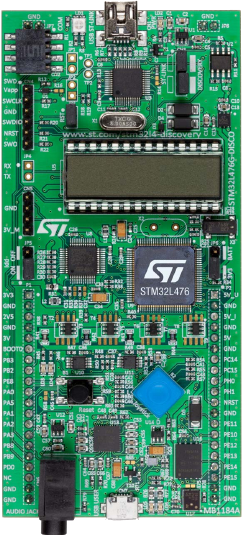
\includegraphics[height=0.3\textheight]{inc/img/discovery}
  \caption{Отладочная плата STM32L476G-Discovery}
  \label{fig:discovery}
\end{figure}

\subsection{Трансивер LoRa}

Модули Semtech LoRa представляют собой ВЧ-трансиверы, с возможностью создания 
топологии M2M (машина-машина) и ``звезда из здвёзд'' (сети LoRa). 
Эти устройства оптимизируют потребление энергии, увеличивая срок службы батарей 
конечных устройств.
Они подробно задокументированы, что делает процесс подключения к интерфейсу
 доступным для широкого круга разработчиков программно-аппаратного обеспечения 
инфраструктуры Интернета вещей.

Серия SX1272/78 имеют бюджет канала в -148 dBm. 
Высокая чувствительность в сочетании с усилителем LNA (малошумящий усилитель)
 +20 дБм обеспечивают надёжную связь для применения в промышленности 
\cite{Rizzi2017}.

\begin{table}[ht]
 \caption{Рабочие частоты для SX1272 и SX1278}
 \begin{tabular}{|c|c|c|}
  \hline
  Устройство & \begin{tabular}[c]{@{}c@{}}Минимальная\\ частота 
  (МГц)\end{tabular} & \begin{tabular}[c]{@{}c@{}}Максимальная\\ частота 
  (МГц)\end{tabular} \\ \hline
  SX1272     & 860                                                               
  & 1020                                                                 \\ 
  \hline
  SX1278     & 137                                                               
  & 525                                                                  \\ 
  \hline
\end{tabular}
 \label{tab:sx127x}
\end{table}

Чувствительность приёмника определяет минимальное значение мощности, которое 
требуется ему для демодуляции и декодирования с целью достижения определенной 
скорости передачи данных. 
Чувствительность обычно выражается в дБм и чем ниже значение, тем лучшую 
чувствительность имеет приёмник, поэтому, исходя из таблицы 
\ref{tab:sx127xParams} можно сделать вывод, что SX1278 имеет большую 
чувствительность приёмника перед SX1272.

\begin{table}[ht]
 \caption{Основные параметры приёмопередатчиков LoRa}
 \begin{tabular}{|c|c|c|c|c|}
\hline
\multirow{2}{*}{\begin{tabular}[c]{@{}c@{}}Приёмо-\\ передатчик\end{tabular}} & 
\multicolumn{4}{c|}{Параметры LoRa}                                              
                                                                                 
                                                                                 
                                                          \\ \cline{2-5} 
                                                                              & 
\begin{tabular}[c]{@{}c@{}}SF \\ диапазон\end{tabular} & 
\begin{tabular}[c]{@{}c@{}}Ширина\\  полосы\\ частот (КГц)\end{tabular} & 
\begin{tabular}[c]{@{}c@{}}Эффективная \\ скорость\\ передачи \\ данных\\ 
(кбит/с)\end{tabular} & \begin{tabular}[c]{@{}c@{}}Чувстви-\\ тельность\\ 
(дБм)\end{tabular} \\ \hline
SX1272                                                                        & 
6..12                                                  & от 125 до 500           
                                                & 0,24..37,5                     
                                                                 & -117..-137    
                                                          \\ \hline
SX1278                                                                        & 
6..12                                                  & от 7,8 до 500           
                                                & 0,018..37,5                    
                                                                 & -111..-148    
                                                          \\ \hline
\end{tabular}
 \label{tab:sx127xParams}
\end{table}

Был выбран приёмопередатчик Semtech SX1278. Выбор был обусловлен тем, что он 
уже имелся в наличии и его внутренняя структура схожа с трансивером SX1272 (они 
имеют общее руководство по эксплуатации).
Данный трансивер будет пригоден для исследовательских работ, но следует иметь в 
виду что для коммерческого использования в России следует выбрать трансивер 
SX1272, поскольку частоты около 868 МГц находятся в пределах поддерживаемых 
частот данного трансивера.

\begin{figure}[!h]
  \centering
  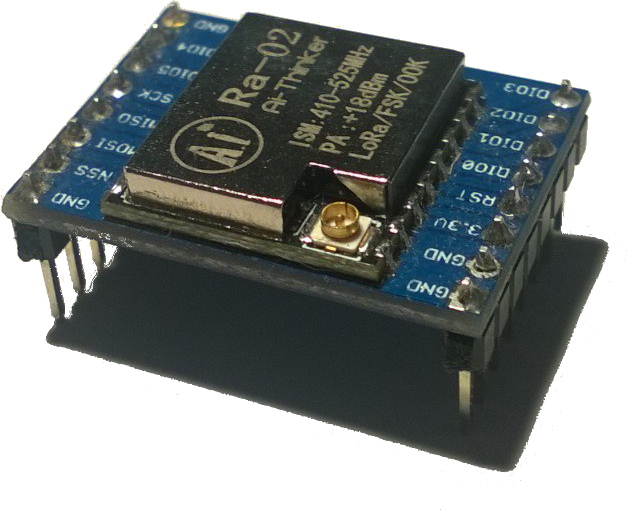
\includegraphics[height=0.3\textheight]{inc/img/SX1278}
  \caption{Трансивер SX1278}
  \label{fig:sx1278}
\end{figure}

Внутренние регистры трансиверов доступны через интерфейс связи SPI.
SPI ""--- это синхронный последовательный полнодуплексный протокол передачи 
данных. 
Обмен по протоколу SPI осуществляют ведущее (\textit{Master}) и подчинённое 
(\textit{Slave}) устройство, приём передачу данных инициирует именно ведущее.

Этот протокол использует 4 линии для связи, которые описываются как:
\begin{itemize}
 \item \textbf{SCLK}. Соответствует тактовому сигналу, генерируется ведущим и 
синхронизирует передачу данных;
 \item \textbf{MOSI} (\textit{Master Out Slave In}). Передача основных данных 
от ведущего к подчиненному устройству;
 \item \textbf{MISO} (\textit{Master In Slave Out}). Передача основных данных 
от подчиненного к ведущему устройству устройству;
 \item $\overline{\text{\textbf{NSS}}}$ (\textit{Slave Select}). Выборка 
%подчиненного устройства. Используется для связи нескольких подчиненных 
%устройств к ведущему. 
\end{itemize}

Радиомодули LoRa работают как подчиненные устройства, а микроконтроллер 
встраиваемой системы будет ведущим в интерфейсе SPI.

На логическом уровне синхронизации и передачи данных для связи SPI требуется 
конфигурация полярности тактирующего сигнала (CPOL) и бит фазы синхронизации 
(CPHA).

Приёмопередатчики LoRa SX1272/78 используют параметры CPOL = 0 и CPHA = 0.
Самый старший бит (MSB) отправленного байта должен быть первым, а скорость SCLK 
не должна превышать 10 МГц.

% Предлагаемая схема соединения здесь?

\section{Описание используемого программного обеспечения}

\subsection{Важность свободного программного обеспечения}

Свободное программное обеспечение играет важную роль для сотрудничества и 
развития поскольку оно обеспечивает технологический суверенитет,
способствует национальным инновациям, оптимизирует расходы на создание 
собственного программного обеспечение, ускоряет местное развитие и 
способствует цифровой интеграции. 

Использование открытого программного обеспечения позволит инфраструктуре 
Интернета вещей:

\begin{itemize}
 \item приобрести технологическую автономию: доступ к исходному коду позволит 
многим пользователям перейти от потребителей к разработчикам программного 
обеспечения;
 \item провести стандартизацию и интеграцию: свободное программное обеспечение 
создается с использованием спецификаций и бесплатных общедоступных 
технологических стандартов, также называемыми ``открытыми стандартами''. Это 
приносит пользу интеграции систем и обмену информацией, гарантирует 
 доступ без ограничений для всех пользователей;
 \item обрести безопасность. Публикация исходных текстов программ или 
приложений способствует их безопасности. Используя открытое программное 
обеспечение, можно узнать и проанализировать, что фактически выполняется 
программой, тип информации, который она обрабатывает и как ей управлять. Хорошая 
безопасность должна основываться на прозрачности. Проприетарное программное 
обеспечение скрывает эти аспекты, и часто неизвестно, сохраняется ли 
конфиденциальность отправляемой информации;
 \item приобрести независимых поставщиков программно-аппаратного обеспечения: 
использование проприетарного программного обеспечения создает зависимость от 
производителя. Как только такое программное обеспечение будет установлено, оно 
будет зависеть от получения обновлений. Во многих случая производитель будет 
принуждать к обновлению до новых версии, даже если это нежелательно.
 \item добиться демократизации информации: информационные технологии заняли 
существенное положение в обществе. Хотя все больше и больше пользователей 
обращаются к указанным технологиям, ``технологический разрыв'' по-прежнему велик 
и является ещё одним фактором социальной изоляции;
 \item добиться экономичности: покупка проприетарного ПО, особенно когда 
производитель имеет монополию на данный вид программного продукта и 
используемых в нём алгоритмов, стоит несравненно больше, чем приобретение и 
использование программного продукта на основе отрытого программного 
обеспечения;
\end{itemize}

\subsection{Основа проекта}

За основу для разработки ПО для микроконтроллера STM32L476VGT6 в связке с 
трансивером SX1278 был взят общедоступный проект от разработчиков альянса LoRa 
Alliance, находящийся по адресу \url{https://github.com/Lora-net/LoRaMac-node} 
(дата обращения 05.06.2018).

Основным используемым языком выбранного проекта является язык программирования 
Си и это не случайно.
Дело в том, что для обеспечения компромисса между производительностью, 
качеством, скоростью, кроссплатформенностью легкостью разработки необходим 
высокоуровневый язык с возможностью кросс-компиляции на различные аппаратные 
платформы и, при этом, он должен иметь наилучшие показатели производительности 
среди всех языков по сравнению с аналогичной программой, написанной на 
ассемблере.
Язык программирования Си удовлетворяет большей части этих требований. 

Однако, для дальнейшего развития инфраструктуры Интернета вещей следует 
исключить из поставщиков услуг разработчиков ПО и предоставить пользователям 
системы возможность самостоятельно, с минимальными знаниями о информационных 
технологиях, изменять программное обеспечение вещей для удовлетворения 
собственных нужд.
Потребуется создание продвинутых визуальных языков программирования и 
предметно-ориентированных языков использующих графическое
представление данных и алгоритмов. 

\subsection{Используемое программное обеспечение}

Для разработки использовались следующее программное обеспечение:
\begin{itemize}
 \item операционная система Linux Kubuntu 17.04;
 \item систему контроля версии Git;
 \item текстовый редактор Vim;
 \item система автоматизации сборки CMake;
 \item утилита автоматизации преобразования файлов make;
 \item утилита прямой отладки программ на микроконтроллере OpenOCD;
 \item отладчик gdb для процессоров ARM;
\end{itemize}


\begin{figure}[!h]
  \centering
  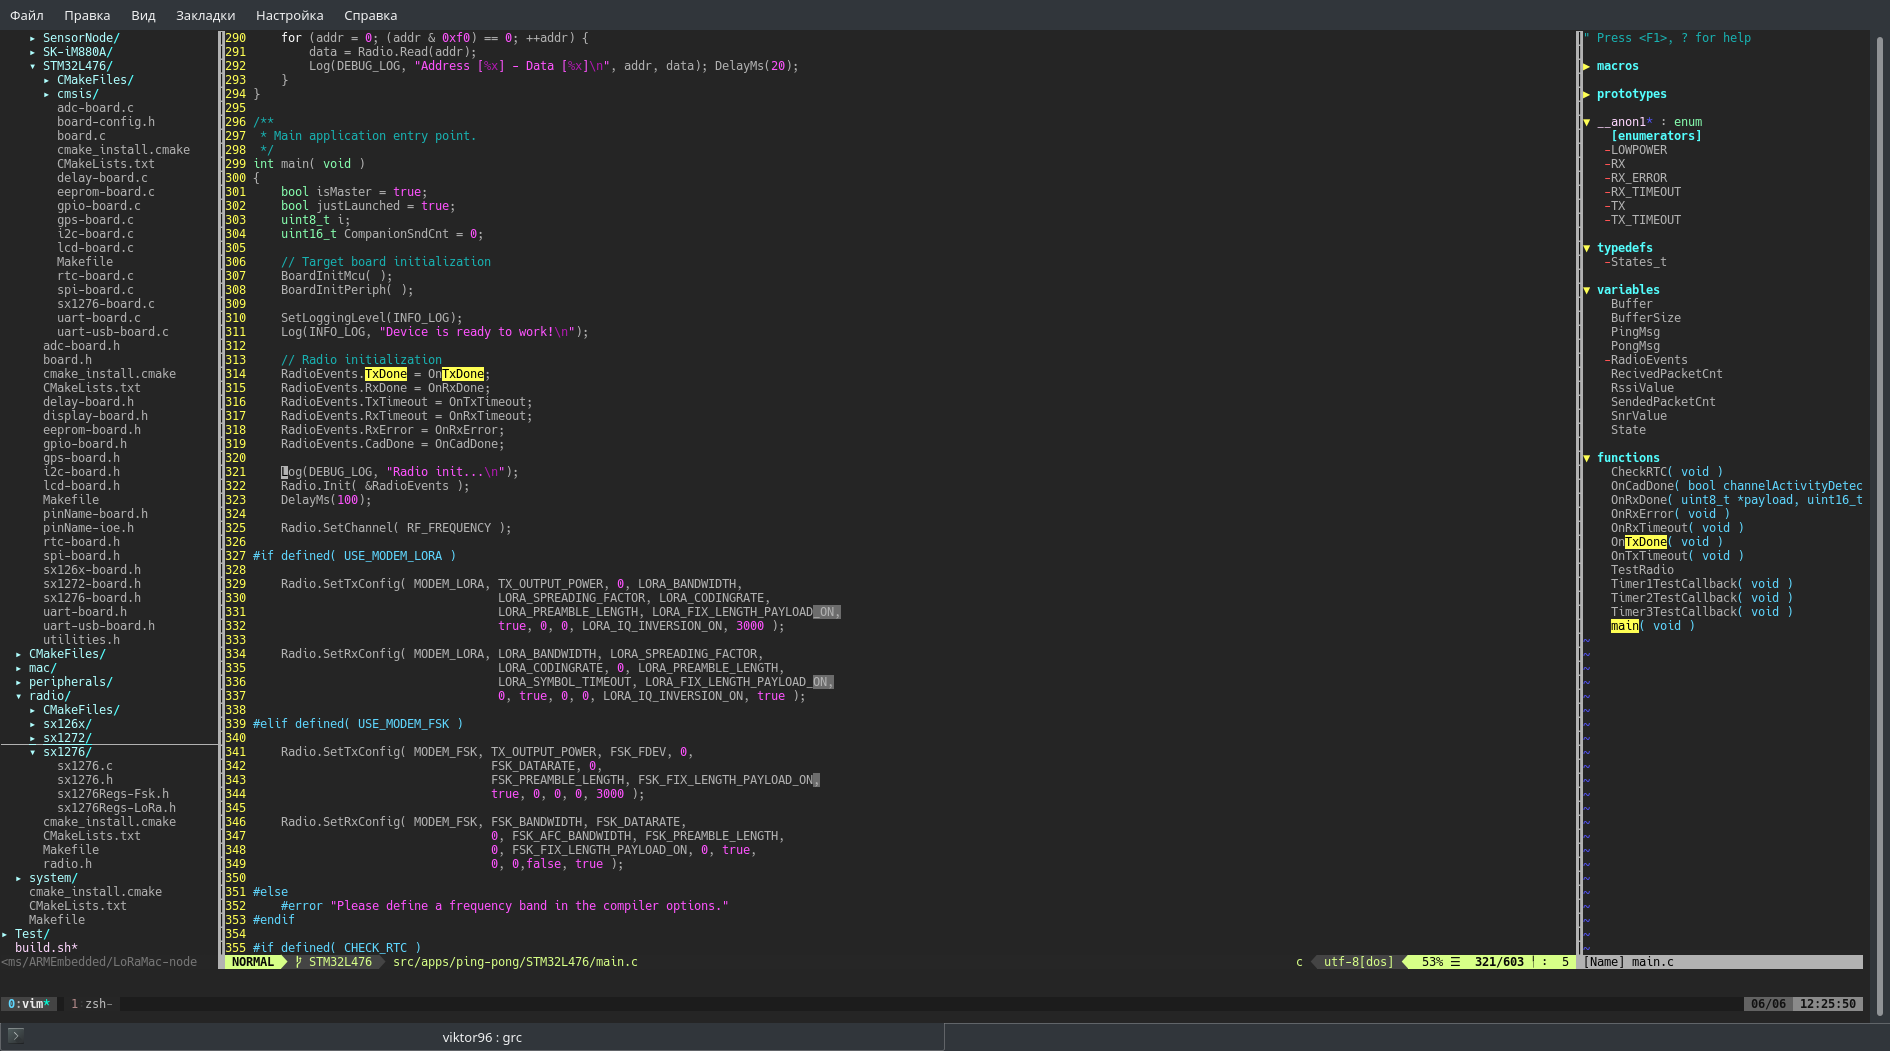
\includegraphics[width=\textwidth]{inc/img/Vim}
  \caption{Текстовый редактор Vim}
  \label{fig:ideeclipse}
\end{figure}

%+Зачем взял LoRaMac на гитхабе
%+Возможно немного слов про открытое ПО
%Ещё чуть чуть про инструменты

\subsubsection{CMake}

CMake ""--- это система сборки кроссплатформенного программного обеспечения из 
исходного кода. 
Она не занимается непосредственной сборкой, а лишь генерирует файлы управления 
сборкой исходя из инструкции в файле CMakeLists.txt.
Такими файлами управления сборкой могут служить файлы Makefile в системах Unix 
для сборки с помощью make, а также проекты XCode для Mac OS X и файлы 
project/solutions (\textit{.sln/.vcxproj/.vcproj}) в \textit{Windows} для 
сборки с помощью Visual C++.

CMake используется в выбранном проекте и пример файла CMakeLists.txt для сборки 
проектов под STM32L4 можно посмотреть в листинге \ref{lst:cmakestm32l4}.

\begin{listing}[H]
% firstline, lastline - какие строки показывать 
\cmakefile[lastline=11]{inc/src/stm32l4.cmake}
\caption{Инструкции для кросс-компиляции кода на платформу STM32L4 (часть 
файла)} 
\label{lst:cmakestm32l4}
\end{listing}

\subsubsection{HAL}

Для разработки программного обеспечения к аппаратной платформе STM32L476VGT6 
решено было использовать слой аппаратных абстракций (HAL), разработанный 
производителями микроконтроллеров семейства STM32 и распространяющийся на 
свободной основе.

HAL предоставляет возможность создания кода, не зависящего от аппаратных 
особенностей выбранной платформы. 
Хотя данный слой написан на языке Си, он реализует в себе множество идей 
объектно-ориентированного программирования (ООП). 
Самой важной идеей разработки такого программного обеспечения, как слой 
аппаратных абстракций, является инкапсуляция.
Инкапсуляция позволяет абстрагироваться от сложности разработки на низком 
уровне, предоставляя удобный интерфейс для написания программ работающих с 
различными устройствами, протоколами передачи данных и т.д.

%\subsection{Выбор компилятора для STM32}

%Раздел в процессе написания...

\subsubsection{ST-LINK/V2 и Openocd}

ST-LINK/V2 является внутрисхемным отладчиком и программатором для отладки 
микроконтроллеров семейства STM32 и STM8.
Данный отладчик спроектирован на базе микроконтроллера STM32F103C8, который 
включает в себя высокопроизводительное ядро ARM-Cortex M3.
Для внутрисхемной отладки он использует JTAG/SWD/SWIM интерфейсы отлаживаемого 
микроконтроллера.

ST-LINK/V2 уже входит в состав отладочной платы STM32L4-Discovery.

OpenOCD ""--- программное обеспечение для ОС Linux, Windows и Mac OS, 
реализующий интерфейс отлаживаемого микроконтроллера через внутрисхемный 
отладчик, такой как ST-LINK/V2 и другие. 
При запуске OpenOCD находит подключенный к компьютеру внутрисхемный отладчик, 
устанавливает с ним связь и открывает локальный TCP сервер, для последующего 
подключения к нему программного отладчика. 
TCP сервер OpenOCD принимает команды от программного отладчика и отсылает их 
внутрисхемному отладчику.
Инструкции подключения OpenOCD к внутрисхемному отладчику отображены в листинге 
\ref{lst:openocdconf}.

\begin{listing}[H]
% firstline, lastline - какие строки показывать 
\textfile{inc/src/openocd.cfg}
\caption{Инструкции подключения OpenOCD к внутрисхемному отладчику} 
\label{lst:openocdconf}
\end{listing}

В качестве программного отладчика была использована утилита arm-none-eabi-gdb, 
конфигурации для подключения можно увидеть в листинге \ref{lst:gdbconf}.

\begin{listing}[H]
% firstline, lastline - какие строки показывать 
\textfile{inc/src/gdb.cfg}
\caption{Инструкции подключения программного отладчика gdb к серверу OpenOCD} 
\label{lst:gdbconf}
\end{listing}

\subsection{Структура проекта LoRaMac}

Код проекта LoRaMAC разбит на несколько пакетов, каждый из которых реализует 
самостоятельный компонент программного обеспечения устройства:
\begin{itemize}
 \item \textit{system} ""--- слой аппаратных абстракций ``система'', 
использующийся пакетами поддержки радиомодулей и алгоритмов MAC. Является 
интерфейсом к используемому аппаратному обеспечению.
 \item \textit{boards} ""--- содержит реализации интерфейса абстракции 
``система'' для каждого вида микроконтроллера;
 \item \textit{radio} ""--- пакет, содержащий интерфейс и реализацию алгоритмов 
и данных для работы с приёмопередатчиками LoRa такими, как SX1272, SX1276, 
SX126x и другими. Для своей работы этот пакет использует слой аппаратных 
абстракции ``система''. 
 \item \textit{mac} ""--- пакет, реализующий данные и алгоритмы работы 
протокола LoRaWAN, включая шифрование данных и регионально-зависимые настройки 
несущих частот и прочих настроек физического уровня LoRa;
 \item \textit{apps} ""--- примеры готовых приложений;
 \item \textit{peripherals} ""--- различные драйверы для периферии, доступной 
на некоторых аппаратных платформах.
\end{itemize}

Упрощенную структуру проекта можно посмотреть на рисунке 
\ref{fig:loramacstructure}.

%Правила переноса кода
\begin{figure}[!h]
  \centering
  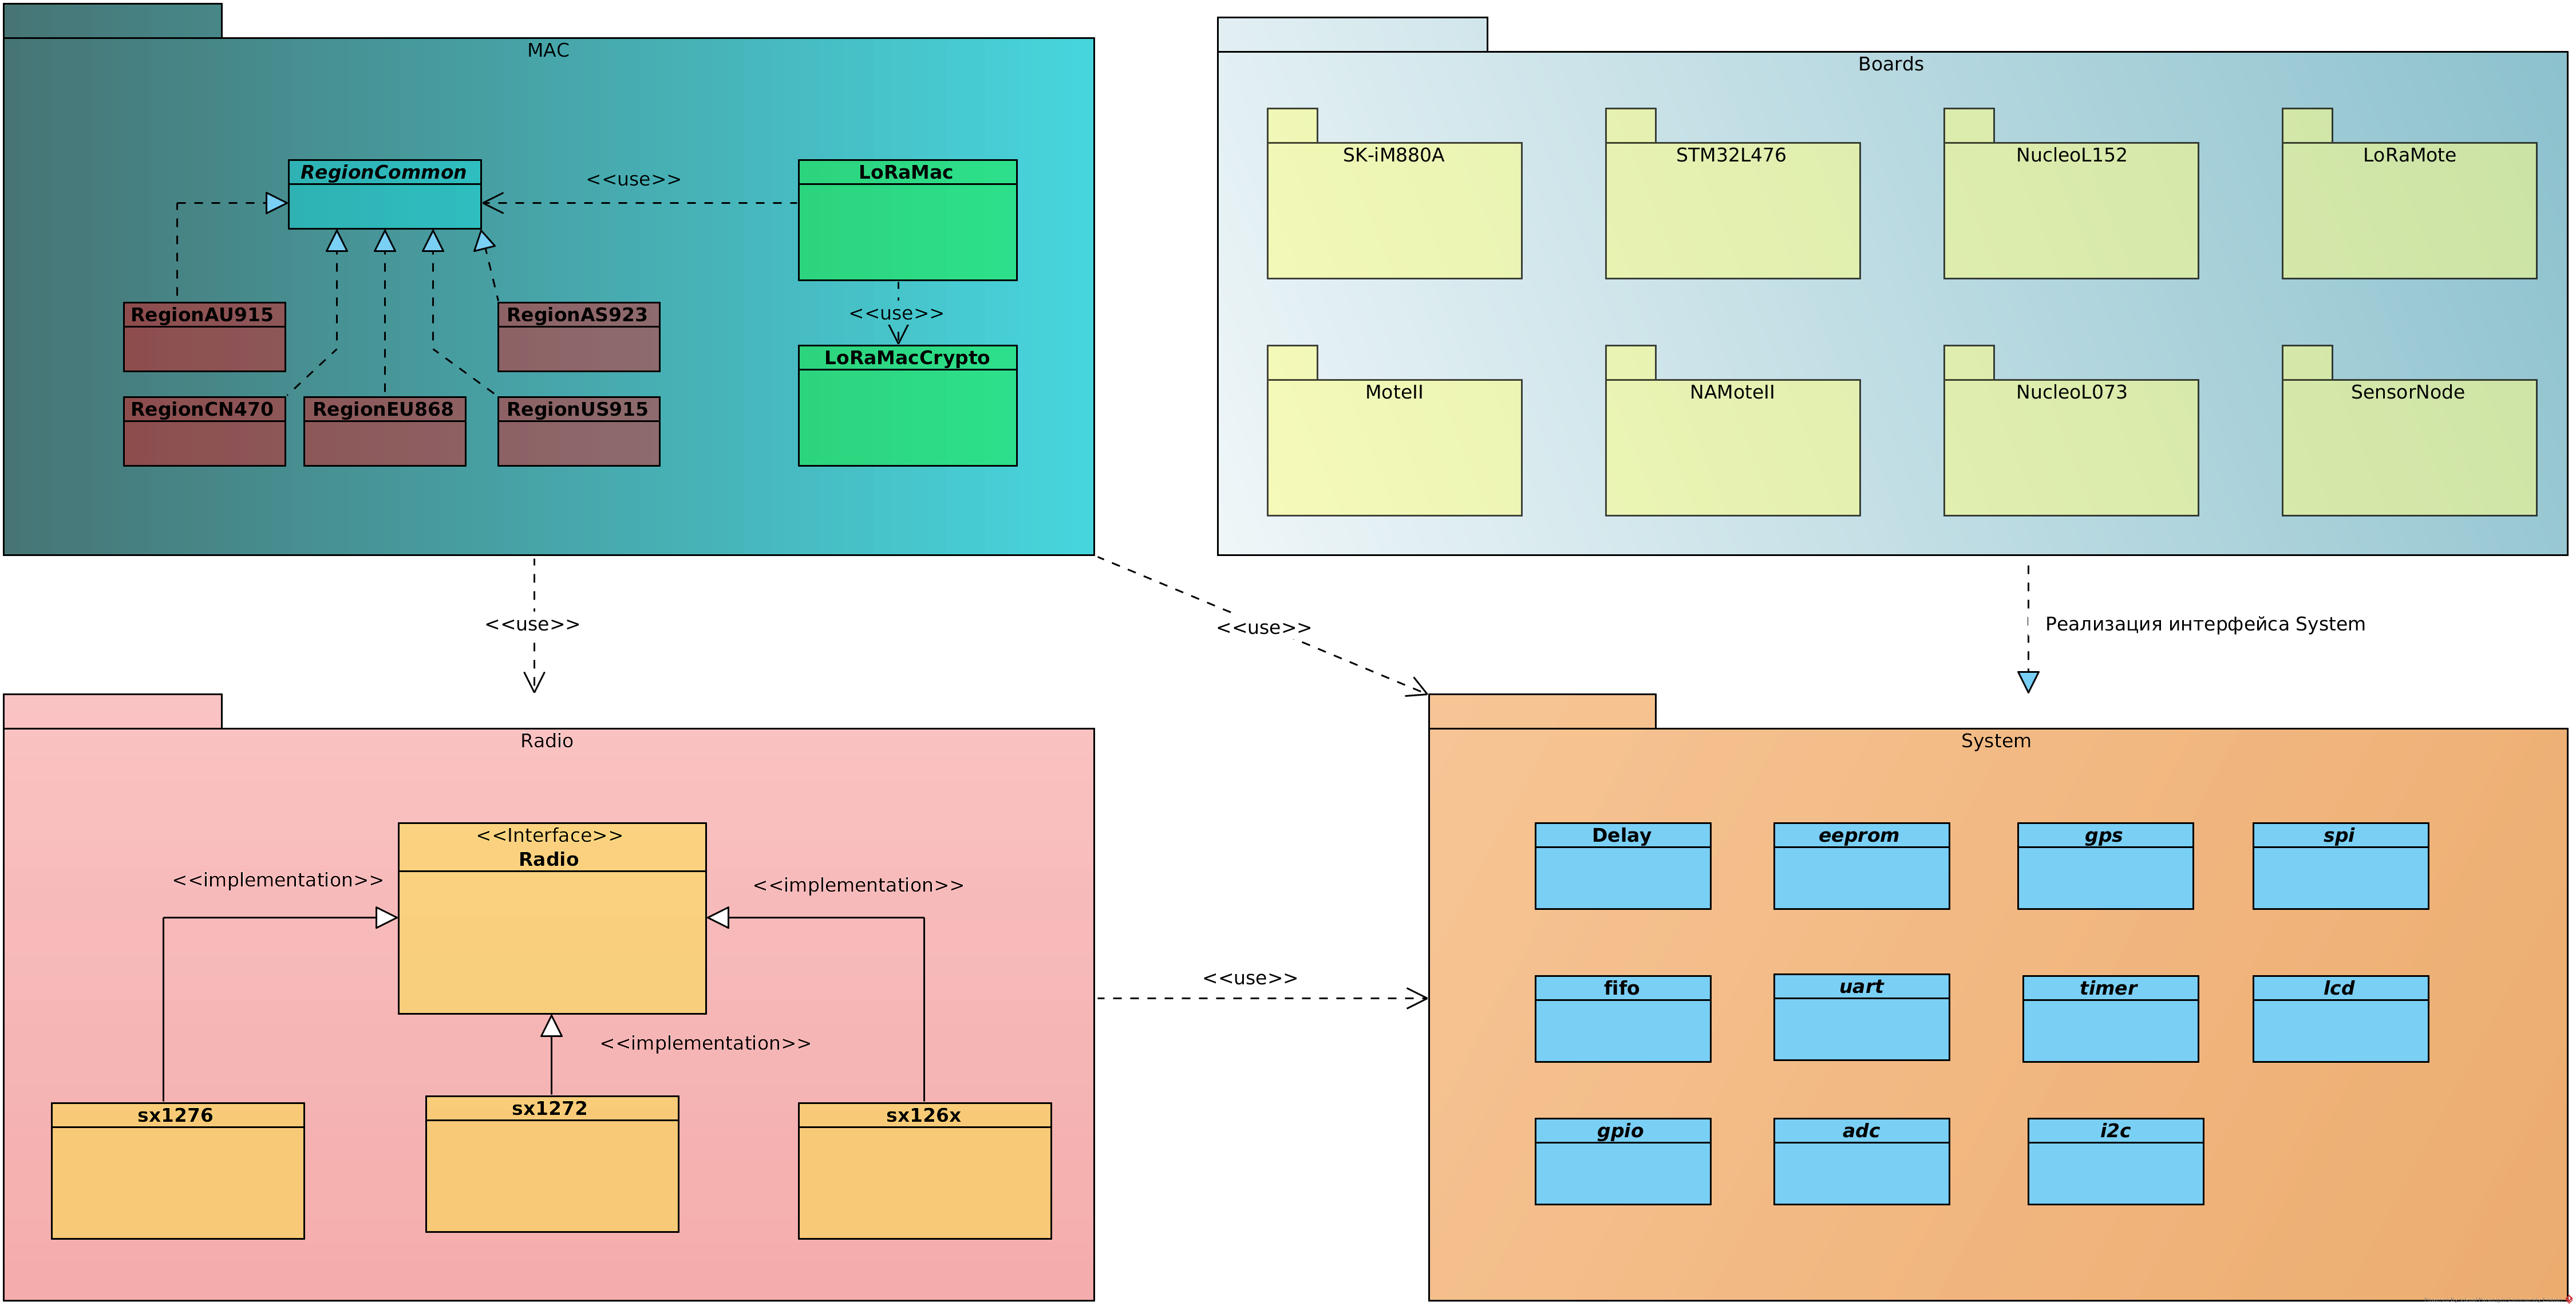
\includegraphics[width=\textwidth]{inc/img/LoRaMacProj}
  \caption{Упрощенная структура проекта LoRaMAC в нотации UML}
  \label{fig:loramacstructure}
\end{figure}

\section{Реализация проекта}

Проект LoRaMAC не содержал в себе исходного кода для реализации связки 
микроконтроллера STM32L476VGT6 на базе ядра ARM Cortex-M4, таким образом 
следовало сперва создать правила компиляции исходного кода для данной 
архитектуры. Эти правила описаны в файле \textit{stm32l4.cmake} и сам файл 
размещён в папке cmake в корне проекта. Часть содержимого этого файла 
отображено на листинге \ref{lst:cmakestm32l4}.

Как можно видеть из листинга, требуется также файл с инструкциями для 
компоновщика под выбранную аппаратную платформу. Код для компоновщика 
поставляется разработчиком аппаратных абстракции HAL.

Далее необходимо:
\begin{enumerate}
 \item добавить новую директорию в пакет \textit{boards} с именем используемой 
аппаратной платформы;
 \item реализовать интерфейс ``системы'' описав следующие модули под 
используемую аппаратную платформу:
 \begin{enumerate}
  \item board.c/.h;
  \item gpio-board.c/.h;
  \item piName-board.c/.h;
  \item piName-ioe.c/.h;
  \item rtc-board.c/.h;
  \item spi-board.c/.h.
 \end{enumerate}
 \item перенести в boards/mcu проект с HAL для STM32L4;
 \item занести конфигурацию оборудования в файл board-config.h.
\end{enumerate}

\subsection{Подключение STM32 к трансиверам LoRa}

Отладочная плата была соединена к интерфейсу SPI пирёмопередатчика SX1278.
Соответствие ножек и их функции приведено в таблице \ref{tab:stm32connect}.

\begin{table}[ht]
 \caption{Соответствие ножек отладочной платы и выполняемой функции}
\begin{tabular}{|c|c|}
\hline
\begin{tabular}[c]{@{}c@{}}Ножка отладочной \\ платы STM32L-DISCO\end{tabular} & 
\begin{tabular}[c]{@{}c@{}}Ножка радиомодуля\\ SX1278\end{tabular} \\ \hline
PE12                                                                           & 
NSS                                                                \\ \hline
PE13                                                                           & 
SCK                                                                \\ \hline
PE14                                                                           & 
MISO                                                               \\ \hline
PE15                                                                           & 
MOSI                                                               \\ \hline
PA5                                                                            & 
DIO0                                                               \\ \hline
PA1                                                                            & 
DIO1                                                               \\ \hline
PA2                                                                            & 
DIO2                                                               \\ \hline
PA3                                                                            & 
DIO3                                                               \\ \hline
PE11                                                                           & 
DIO4                                                               \\ \hline
PE10                                                                           & 
DIO5                                                               \\ \hline
PB7                                                                            & 
RESET                                                              \\ \hline
\end{tabular}
 \label{tab:stm32connect}
\end{table}

Собранный прототип отображен на рисунке \ref{fig:stm32lora}.

\begin{figure}[!h]
  \centering
  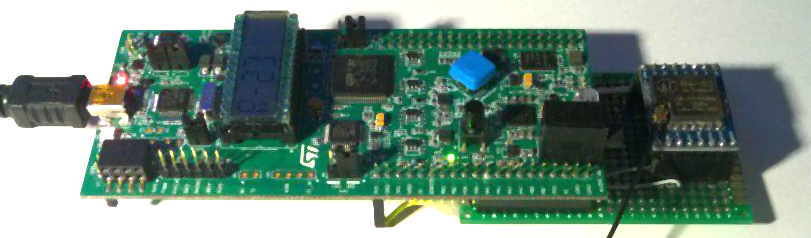
\includegraphics[width=\textwidth]{inc/img/stm32lora}
  \caption{Собранный прототип конечного устройства}
  \label{fig:stm32lora}
\end{figure}
% Желательно схему

\subsection{Сложности переноса}

Во время переноса кода на новую аппаратную платформу пришлось разрешить 
некоторые проблемы.
Во-первых, слой аппаратных абстракции не рассматривает использование новой
архитектуры ARM Cortex-M4, приходилось подбирать верные ключи для 
кросс-компиляции. 
Во-вторых, также не предполагалось использование SX1278, поэтому пришлось 
перенастроить частотные используемые частотные диапазоны в исходных файлах.
В-третьих, сам слой аппаратных абстракции содержит ошибки (неточности) в 
выбранных типах данных для интерфейсов.
Поскольку эти типы данных основаны на HAL, а HAL сам меняется, то в слое 
аппаратных абстракций LoRaMAC возникают множество неприятных ловушек, связанных 
с использование старой версии HAL.

Приведу конкретный пример: во время инициализации интерфейса SPI вызывалась 
функция выбора формата сигнала SPI ""--- \texttt{SpiFormat}:

\begin{minted}[linenos,breaklines,frame=single]{c}
if( nss == NC )
{
    SpiHandle[spiId].Init.NSS = SPI_NSS_SOFT;
    SpiFormat( obj, SPI_DATASIZE_8BIT, SPI_POLARITY_LOW, SPI_PHASE_1EDGE, 0 );
}
else
{
    SpiFormat( obj, SPI_DATASIZE_8BIT, SPI_POLARITY_LOW, SPI_PHASE_1EDGE, 1 );
}
\end{minted}

Второй параметр определяет сколько бит данных должен передавать один кадр SPI 
(в момент времени когда на линии \textit{NSS} логическая единица).
Готовый интерфейс аппаратных абстракций содержит следующее определение:
\begin{minted}[linenos,breaklines,frame=single]{c}
 /*!
 * \brief Configures the SPI peripheral
 *
 * \remark Slave mode isn't currently handled
 *
 * \param [IN] obj   SPI object
 * \param [IN] bits  Number of bits to be used. [8 or 16]
 * \param [IN] cpol  Clock polarity
 * \param [IN] cpha  Clock phase
 * \param [IN] slave When set the peripheral acts in slave mode
 */
void SpiFormat( Spi_t *obj, int8_t bits, int8_t cpol, int8_t cpha, int8_t slave 
);
\end{minted}

Здесь второй параметр определен как 8-битное целое число. 
Видимо первоначально предполагалось что туда будет передаваться всего два 
возможных значения ""--- \texttt{SPI\_DATASIZE\_8BIT} и 
\texttt{SPI\_DATASIZE\_16BIT}.
Так оно и было в старой версии HAL, однако в новой версии HAL для STM32L4 
добавились новые значения:

\begin{minted}[linenos,breaklines,frame=single]{c}
/** @defgroup SPI_Data_Size SPI Data Size            
  * @{                                               
  */                                                 
#define SPI_DATASIZE_4BIT               (0x00000300U)
#define SPI_DATASIZE_5BIT               (0x00000400U)
#define SPI_DATASIZE_6BIT               (0x00000500U)
#define SPI_DATASIZE_7BIT               (0x00000600U)
#define SPI_DATASIZE_8BIT               (0x00000700U)
#define SPI_DATASIZE_9BIT               (0x00000800U)
#define SPI_DATASIZE_10BIT              (0x00000900U)
#define SPI_DATASIZE_11BIT              (0x00000A00U)
#define SPI_DATASIZE_12BIT              (0x00000B00U)
#define SPI_DATASIZE_13BIT              (0x00000C00U)
#define SPI_DATASIZE_14BIT              (0x00000D00U)
#define SPI_DATASIZE_15BIT              (0x00000E00U)
#define SPI_DATASIZE_16BIT              (0x00000F00U)
\end{minted}

Как можно видеть теперь младший байт для передачи значения не используется, что 
приводило к неоднозначной ошибке исполнения программы: программа продолжала 
выполнятся, а SPI передавал 16 бит вместо 8. 
Ушло примерно два часа на анализ пока ошибка не была найдена и теперь 
определение функции выглядит так:

\begin{minted}[linenos,breaklines,frame=single]{c}
void SpiFormat( Spi_t *obj, int32_t bits, int8_t cpol, int8_t cpha, int8_t 
slave 
);
\end{minted}

Ошибка была исправлена. 
Безусловно подобные ошибки происходят не только по вине человека, но и по 
несовершенству средств программирования.
Язык Си является языком с, так называемой, мягкой типизацией, которая позволяет 
таким ошибкам происходить совершенно незаметно для разработчика.


%\begin{listing}[H]
% firstline, lastline - какие строки показывать 
%\cfile{inc/src/test.c}
%\caption{Пример — test.c} 
%\end{listing}
%\label{lst:c}

%Можно также использовать окружение \Code{verbatim}, если \Code{listings} чем-то не
%устраивает. Только следует помнить, что табы в нём <<съедаются>>. Существует так же команда \Code{\textbackslash{}verbatiminput} для вставки файла.

%\begin{verbatim}
%a_b = a + b; // русский комментарий
%if (a_b > 0)
    %a_b = 0;
%\end{verbatim}

%%% Local Variables:
%%% mode: latex
%%% TeX-master: "rpz"
%%% End:

\chapter{Проверка работы устройства}
\label{cha:pract}

\section{Ping-Pong}

Было собрано два идентичных устройства и портирован код приложения Ping-Pong, 
являющийся в беспроводных приложениях подобием доказательства концепции 
(\textit{proof of concept}).

Приложение было модернизировано, добавление системы логирования и счётчиками 
отправленных и принятых пакетов.
Логирование осуществлялась посредством виртуального COM интерфейса STM32L4.
Во время подключения к компьютеру плата отправляет через COM интерфейс 
отладочные данные. 
Пример отладочных данных дан ниже:
\textfile[firstline=6,lastline=11]{inc/src/N61.76196E34.36578.txt}

Полный исходный код приложения Ping-Pong будет дан в приложении 
\ref{cha:appendix1}.

\section{Проверка работы приёмопередатчиков}

Была установлена связь с между модулями и переданы кадры с содержимым
``ping'' и ``pong''.
Используемые параметры физического уровня: модуляция LoRa, SF = 7, BW = 125 
кГц, несущая частота равна 433 МГц, CR = 4/5, длина преамбулы равна 8, усиление 
передатчика - 14 дБ.
Использовалась антенна с усилением 4 дБ.

%\begin{figure}[!h]
  %\centering
  %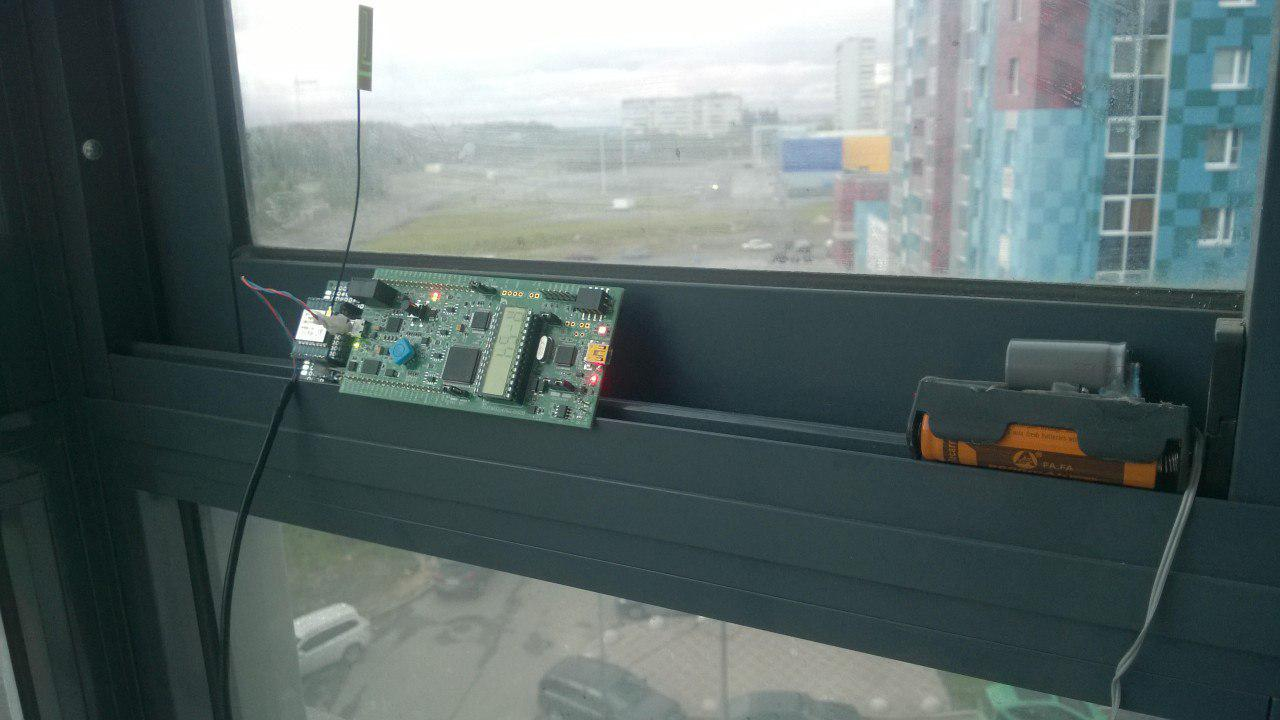
\includegraphics[width=\textwidth]{inc/img/exp1}
  %\caption{Автономное устройство, передающее кадры Ping в приложении Ping-Pong}
  %\label{fig:exp1}
%\end{figure}

%Результаты измерений отображены на рисунке \ref{fig:measmap} и в таблице 
%\ref{tab:meastab}.

%\begin{table}[ht]
%  \caption{Результаты замеров}
%  \begin{tabular}{|l|c|c|c|}
%\hline
%\begin{tabular}[c]{@{}l@{}}Описание \\ места\end{tabular}                        
%                & \begin{tabular}[c]{@{}c@{}}Расстояние \\ до БС, м\end{tabular} 
%& PER, \%      & RSSI, дБм                                                  \\ 
%\hline
%\begin{tabular}[c]{@{}l@{}}За домом.\\ Несколько стен.\end{tabular}              
%                & 40                                                             
%& 0,8 & -94                                                   \\ \hline
%\begin{tabular}[c]{@{}l@{}}Улица.\\ Прямая видимость БС\end{tabular}          
%                & 293                                                            
%& 1            & -88                                                   \\ \hline
%\begin{tabular}[c]{@{}l@{}}В магазине\\ Видимости нет.\\ Глубоко 
%внутри помещения\end{tabular} & 280                                              
%              & 100          & \begin{tabular}[c]{@{}c@{}}Нет\\ 
%сигнала\end{tabular} \\ \hline
%\begin{tabular}[c]{@{}l@{}}Улица.\\ Прямой\\ видимости нет.\\ Рельеф 
%закрывает БС\end{tabular} & 687                                                  
%          & 14,9         & -102                                                 
% \\ \hline
%\begin{tabular}[c]{@{}l@{}}Улица. Прямой \\ видимости нет. \\ Плотная 
%застройка.\end{tabular}    & 524                                                 
%           & 24,4         & -112                                                 
% \\ \hline
%\end{tabular}
%  \label{tab:meastab}
%\end{table}
%

%begin{figure}[!h]
  %\centering
  %%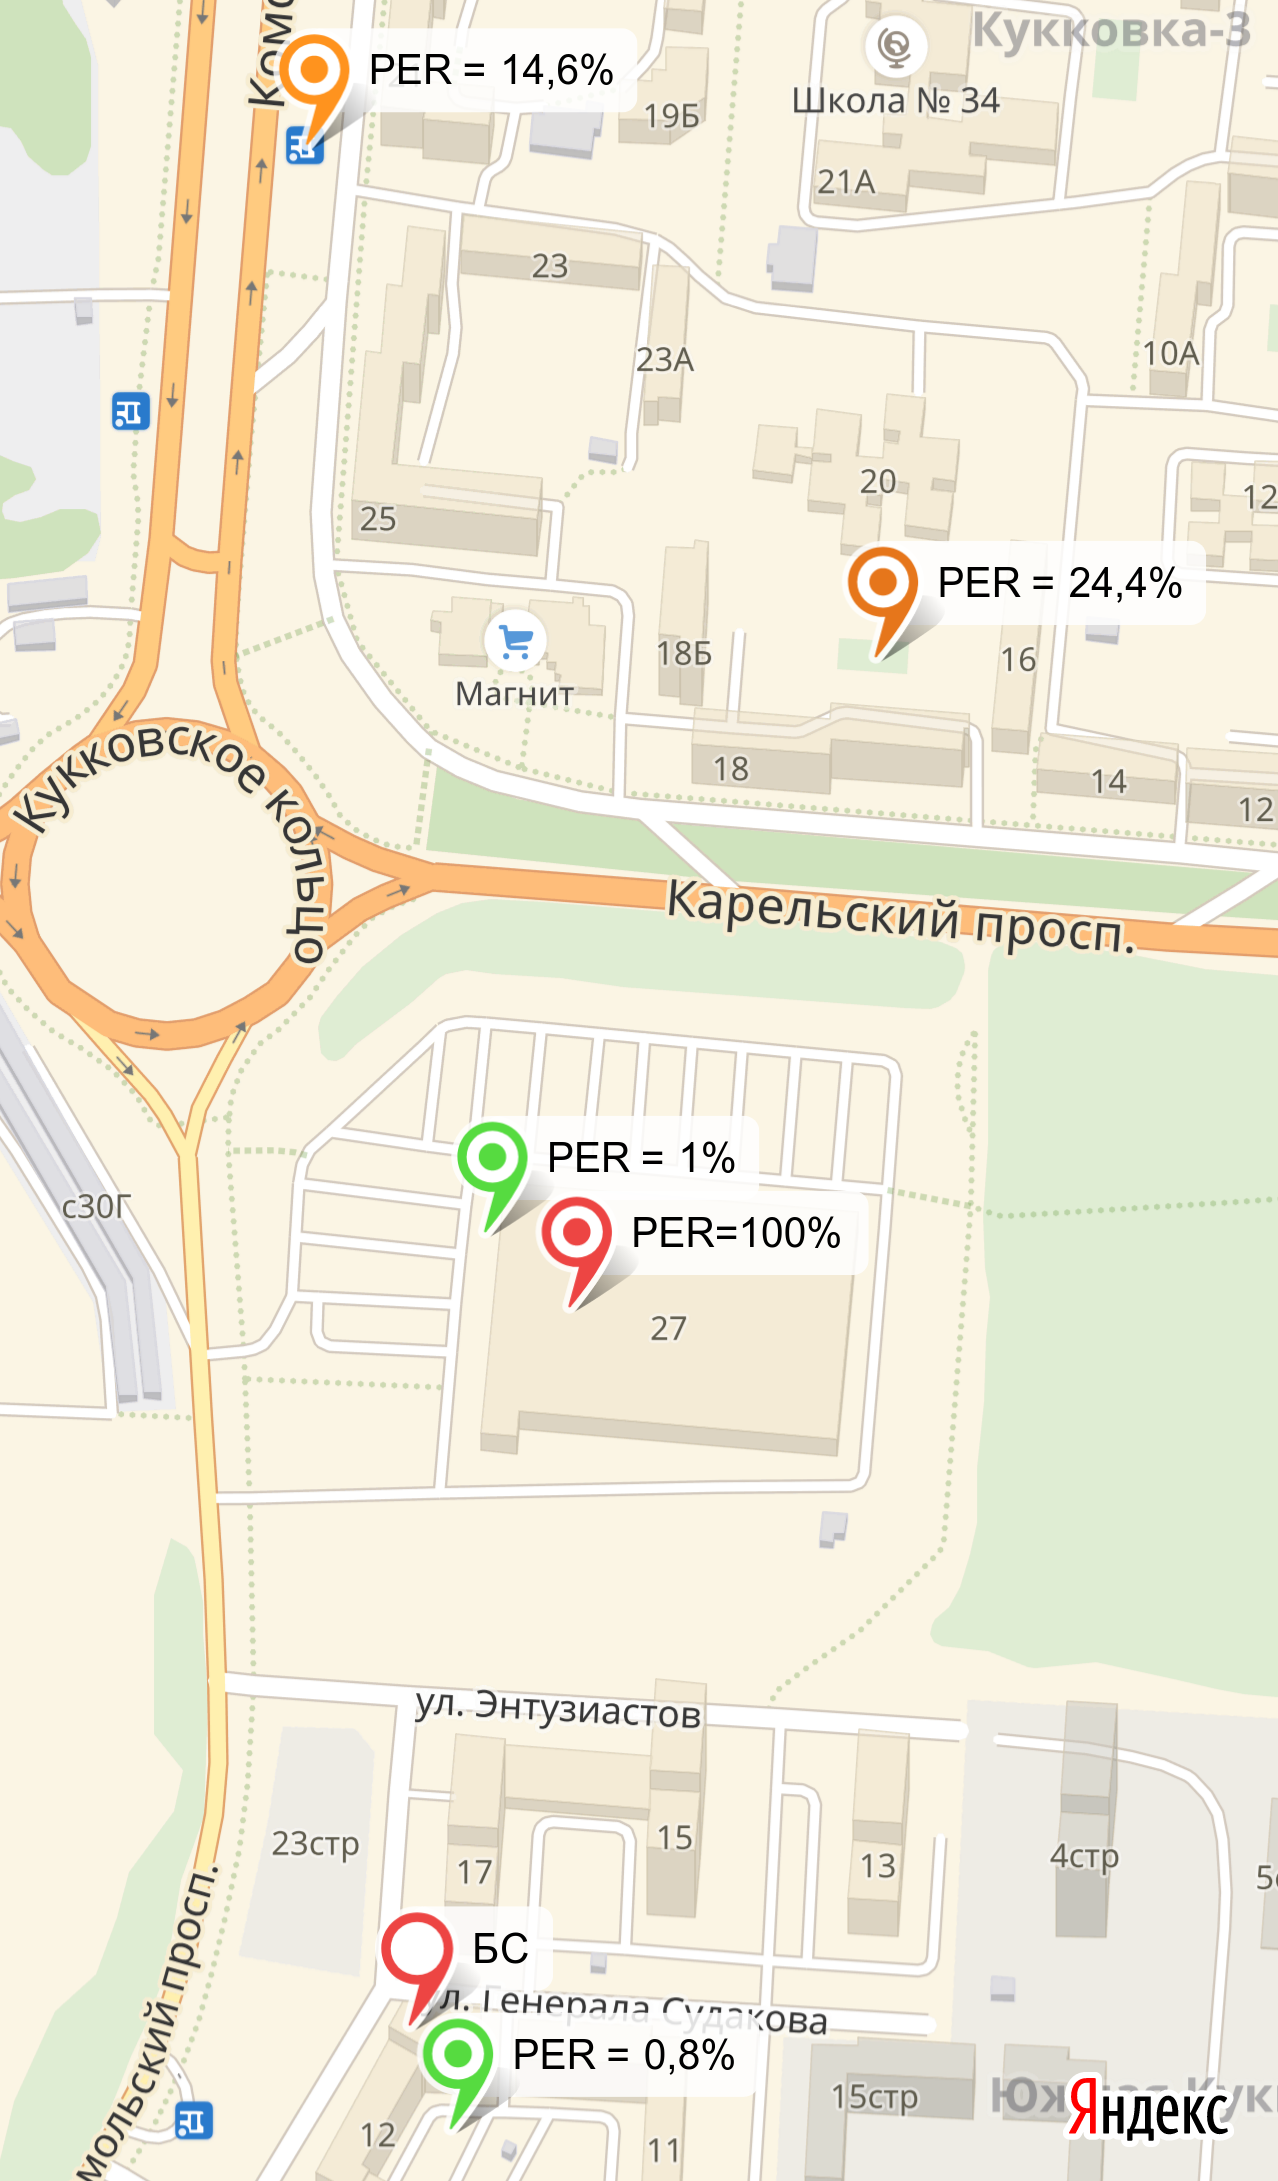
\includegraphics[height=0.9\textheight]{inc/img/LoRaMeas}
  %\caption{Результаты замеров качества приёма пакетов}
  %\label{fig:measmap}
%\end{figure}


\backmatter %% Здесь заканчивается нумерованная часть документа и начинаются ссылки и
            
\Conclusion % заключение к отчёту

В ходе исследования LoRa в контексте её использования для построения сети 
Интернета вещей, были выполнены следующие задачи:

\begin{itemize}
 \item оценены достоинства и недостатки применения данной технологии для 
построения LPWAN сетей;
 \item рассмотрен и предложен ряд вариантов использования данной технологии с 
поправкой на её особенности в концепции Интернета вещей.
 \item было разработано программное обеспечение для сопряжения STM32L4 с 
трансивервами LoRa;
 \item разработанное ПО было задокументировано и выложено в открытый доступ;
\end{itemize}

Был приобретён навык работы с исходными кодами программного обеспечения, 
распространяющегося на свободной основе.
Также приобретён навык переноса исходного кода на новую аппаратную платформу, 
что немаловажно для создания кросс-платформенного ПО, которое станет основой 
для инфраструктуры Интернета вещей.

%%% Local Variables: 
%%% mode: latex
%%% TeX-master: "rpz"
%%% End: 
%% заключение

% % Список литературы при помощи BibTeX
% Юзать так:
%
% pdflatex rpz
% bibtex rpz
% pdflatex rpz

\bibliographystyle{ugost2008}
\bibliography{rpz}

%%% Local Variables: 
%%% mode: latex
%%% TeX-master: "rpz"
%%% End: 


\appendix   % Тут идут приложения

\chapter{Картинки}
\label{cha:appendix1}

\blindtext
\begin{figure}
\centering
\caption{Картинка в приложении. Страшная и ужасная.}
\end{figure}

%%% Local Variables: 
%%% mode: latex
%%% TeX-master: "rpz"
%%% End: 


%\chapter{Еще картинки}
\label{cha:appendix2}
\blindtext

\begin{figure}
\centering
\caption{Еще одна картинка, ничем не лучше предыдущей. Но надо же как-то заполнить место.}
\end{figure}

%%% Local Variables: 
%%% mode: latex
%%% TeX-master: "rpz"
%%% End: 


\end{document}

%%% Local Variables:
%%% mode: latex
%%% TeX-master: t
%%% End:
